%%%%%%%%%%%%%%%%%%%%%%%%%%%%%%%%%%%%%%%%%
% The Legrand Orange Book
% LaTeX Template
% Version 1.2 (19/5/13)
%
% This template has been downloaded from:
% http://www.LaTeXTemplates.com
%
% Original author:
% Mathias Legrand (legrand.mathias@gmail.com)
%
% License:
% CC BY-NC-SA 3.0 (http://creativecommons.org/licenses/by-nc-sa/3.0/)
%
% Compiling this template:
% This template uses biber for its bibliography and makeindex for its index.
% This means that to update the bibliography and index in this template you
% will need to run the following sequence of commands in the template
% directory:
%
% 1) pdflatex main
% 2) makeindex main.idx -s StyleInd.ist
% 3) biber main
% 4) pdflatex main
%
% This template also uses a number of packages which may need to be
% updated to the newest versions for the template to compile. It is strongly
% recommended you update your LaTeX distribution if you have any
% compilation errors.
%
% Important note:
% Chapter heading images should have a 2:1 width:height ratio,
% e.g. 920px width and 460px height.
%
%%%%%%%%%%%%%%%%%%%%%%%%%%%%%%%%%%%%%%%%%

%----------------------------------------------------------------------------------------
%	PACKAGES AND OTHER DOCUMENT CONFIGURATIONS
%----------------------------------------------------------------------------------------

\documentclass[11pt,fleqn]{book} % Default font size and left-justified equations

\usepackage[top=3cm,bottom=3cm,left=3.2cm,right=3.2cm,headsep=10pt,a4paper]{geometry} % Page margins

\usepackage{xcolor} % Required for specifying colors by name
%\definecolor{ocre}{RGB}{243,102,25} % Define the orange color used for highlighting throughout the book
\definecolor{ocre}{RGB}{57,190,171}

% Font Settings
\usepackage{avant} % Use the Avantgarde font for headings
%\usepackage{times} % Use the Times font for headings
\usepackage{mathptmx} % Use the Adobe Times Roman as the default text font together with math symbols from the Sym­bol, Chancery and Com­puter Modern fonts

\usepackage{microtype} % Slightly tweak font spacing for aesthetics

% Index
\usepackage{calc} % For simpler calculation - used for spacing the index letter headings correctly
\usepackage{makeidx} % Required to make an index
\makeindex % Tells LaTeX to create the files required for indexing

%----------------------------------------------------------------------------------------

%----------------------------------------------------------------------------------------
%	VARIOUS REQUIRED PACKAGES
%----------------------------------------------------------------------------------------

\usepackage{titlesec} % Allows customization of titles

\usepackage{graphicx} % Required for including pictures
\graphicspath{{./Pictures/}} % Specifies the directory where pictures are stored

\usepackage{lipsum} % Inserts dummy text

\usepackage{tikz} % Required for drawing custom shapes

\usepackage[spanish]{babel} % English language/hyphenation

\usepackage{enumitem} % Customize lists
\setlist{nolistsep} % Reduce spacing between bullet points and numbered lists

\usepackage{booktabs} % Required for nicer horizontal rules in tables

\usepackage{eso-pic} % Required for specifying an image background in the title page

%----------------------------------------------------------------------------------------
%	MAIN TABLE OF CONTENTS
%----------------------------------------------------------------------------------------

\usepackage{titletoc} % Required for manipulating the table of contents

\contentsmargin{0cm} % Removes the default margin
% Chapter text styling
\titlecontents{chapter}[1.25cm] % Indentation
{\addvspace{15pt}\large\sffamily\bfseries} % Spacing and font options for chapters
{\color{ocre!60}\contentslabel[\Large\thecontentslabel]{1.25cm}\color{ocre}} % Chapter number
{}
{\color{ocre!60}\normalsize\sffamily\bfseries\;\titlerule*[.5pc]{.}\;\thecontentspage} % Page number
% Section text styling
\titlecontents{section}[1.25cm] % Indentation
{\addvspace{5pt}\sffamily\bfseries} % Spacing and font options for sections
{\contentslabel[\thecontentslabel]{1.25cm}} % Section number
{}
{\sffamily\hfill\color{black}\thecontentspage} % Page number
[]
% Subsection text styling
\titlecontents{subsection}[1.25cm] % Indentation
{\addvspace{1pt}\sffamily\small} % Spacing and font options for subsections
{\contentslabel[\thecontentslabel]{1.25cm}} % Subsection number
{}
{\sffamily\;\titlerule*[.5pc]{.}\;\thecontentspage} % Page number
[]

%----------------------------------------------------------------------------------------
%	MINI TABLE OF CONTENTS IN CHAPTER HEADS
%----------------------------------------------------------------------------------------

% Section text styling
\titlecontents{lsection}[0em] % Indendating
{\footnotesize\sffamily} % Font settings
{}
{}
{}

% Subsection text styling
\titlecontents{lsubsection}[.5em] % Indentation
{\normalfont\footnotesize\sffamily} % Font settings
{}
{}
{}

%----------------------------------------------------------------------------------------
%	PAGE HEADERS
%----------------------------------------------------------------------------------------

\usepackage{fancyhdr} % Required for header and footer configuration

\pagestyle{fancy}
\renewcommand{\chaptermark}[1]{\markboth{\sffamily\normalsize\bfseries #1}{}} % Chapter text font settings
\renewcommand{\sectionmark}[1]{\markright{\sffamily\normalsize\thesection\hspace{5pt}#1}{}} % Section text font settings
\fancyhf{} \fancyhead[LE,RO]{\sffamily\normalsize\thepage} % Font setting for the page number in the header
\fancyhead[LO]{\rightmark} % Print the nearest section name on the left side of odd pages
\fancyhead[RE]{\leftmark} % Print the current chapter name on the right side of even pages
\renewcommand{\headrulewidth}{0.5pt} % Width of the rule under the header
\addtolength{\headheight}{2.5pt} % Increase the spacing around the header slightly
\renewcommand{\footrulewidth}{0pt} % Removes the rule in the footer
\fancypagestyle{plain}{\fancyhead{}\renewcommand{\headrulewidth}{0pt}} % Style for when a plain pagestyle is specified

% Removes the header from odd empty pages at the end of chapters
\makeatletter
\renewcommand{\cleardoublepage}{
\clearpage\ifodd\c@page\else
\hbox{}
\vspace*{\fill}
\thispagestyle{empty}
\newpage
\fi}

%----------------------------------------------------------------------------------------
%	THEOREM STYLES
%----------------------------------------------------------------------------------------

\usepackage{amsmath,amsfonts,amssymb,amsthm} % For including math equations, theorems, symbols, etc

\newcommand{\intoo}[2]{\mathopen{]}#1\,;#2\mathclose{[}}
\newcommand{\ud}{\mathop{\mathrm{{}d}}\mathopen{}}
\newcommand{\intff}[2]{\mathopen{[}#1\,;#2\mathclose{]}}
\newtheorem{notation}{Notation}[chapter]

\newtheoremstyle{ocrenum} % Theorem style name
{7pt} % Space above
{7pt} % Space below
{\normalfont} % Body font
{} % Indent amount
{\small\bf\sffamily\color{ocre}} % Theorem head font
{\;\;} % Punctuation after theorem head
{0.25em} % Space after theorem head
{\small\sffamily\color{ocre}\thmname{#1}\thmnumber{\@ifnotempty{#1}{ }\@upn{#2}} % Theorem text (e.g. Theorem 2.1)
\thmnote{\ {\the\thm@notefont\sffamily\bfseries\color{black}--- #3.}}} % Optional theorem note
\renewcommand{\qedsymbol}{$\blacksquare$} % Optional qed square

\newtheoremstyle{blacknumex} % Theorem style name
{7pt} % Space above
{7pt} % Space below
{\normalfont} % Body font
{} % Indent amount
{\small\bf\sffamily} % Theorem head font
{\;\;} % Punctuation after theorem head
{0.25em} % Space after theorem head
{\small\sffamily{\tiny\ensuremath{\blacksquare}}\ \thmname{#1}\thmnumber{\@ifnotempty{#1}{ }\@upn{#2}} % Theorem text (e.g. Theorem 2.1)
\thmnote{\ {\the\thm@notefont\sffamily\bfseries--- #3.}}} % Optional theorem note

\newtheoremstyle{blacknum} % Theorem style name
{7pt} % Space above
{7pt} % Space below
{\normalfont} % Body font
{} % Indent amount
{\small\bf\sffamily} % Theorem head font
{\;\;} % Punctuation after theorem head
{0.25em} % Space after theorem head
{\small\sffamily\thmname{#1}\thmnumber{\@ifnotempty{#1}{ }\@upn{#2}} % Theorem text (e.g. Theorem 2.1)
\thmnote{\ {\the\thm@notefont\sffamily\bfseries--- #3.}}} % Optional theorem note
\makeatother

% Defines the theorem text style for each type of theorem to one of the three styles above
\theoremstyle{ocrenum}
\newtheorem{theoremeT}{Theorem}[chapter]
\newtheorem{proposition}{Proposition}[chapter]
\newtheorem{problem}{Problem}[chapter]
\newtheorem{exerciseT}{Exercise}[chapter]
\theoremstyle{blacknumex}
\newtheorem{exampleT}{Example}[chapter]
\theoremstyle{blacknum}
\newtheorem{vocabulary}{Vocabulary}[chapter]
\newtheorem{definitionT}{Definition}[chapter]
\newtheorem{corollaryT}{Corollary}[chapter]

%----------------------------------------------------------------------------------------
%	DEFINITION OF COLORED BOXES
%----------------------------------------------------------------------------------------

\RequirePackage[framemethod=default]{mdframed} % Required for creating the theorem, definition, exercise and corollary boxes

% Theorem box
\newmdenv[skipabove=7pt,
skipbelow=7pt,
backgroundcolor=black!5,
linecolor=ocre,
innerleftmargin=5pt,
innerrightmargin=5pt,
innertopmargin=5pt,
leftmargin=0cm,
rightmargin=0cm,
innerbottommargin=5pt]{tBox}

% Exercise box
\newmdenv[skipabove=7pt,
skipbelow=7pt,
rightline=false,
leftline=true,
topline=false,
bottomline=false,
backgroundcolor=ocre!10,
linecolor=ocre,
innerleftmargin=5pt,
innerrightmargin=5pt,
innertopmargin=5pt,
innerbottommargin=5pt,
leftmargin=0cm,
rightmargin=0cm,
linewidth=4pt]{eBox}

% Definition box
\newmdenv[skipabove=10pt,
skipbelow=10pt,
rightline=false,
leftline=true,
topline=false,
bottomline=false,
linecolor=ocre,
innerleftmargin=5pt,
innerrightmargin=5pt,
innertopmargin=0pt,
leftmargin=0cm,
rightmargin=0cm,
linewidth=4pt,
innerbottommargin=0pt]{dBox}

% Corollary box
\newmdenv[skipabove=7pt,
skipbelow=7pt,
rightline=false,
leftline=true,
topline=false,
bottomline=false,
linecolor=gray,
backgroundcolor=black!5,
innerleftmargin=5pt,
innerrightmargin=5pt,
innertopmargin=5pt,
leftmargin=0cm,
rightmargin=0cm,
linewidth=4pt,
innerbottommargin=5pt]{cBox}


% Creates an environment for each type of theorem and assigns it a theorem text style from the "Theorem Styles" section above and a colored box from above
\newenvironment{theorem}{\begin{tBox}\begin{theoremeT}}{\end{theoremeT}\end{tBox}}
\newenvironment{exercise}{\begin{eBox}\begin{exerciseT}}{\hfill{\color{ocre}\tiny\ensuremath{\blacksquare}}\end{exerciseT}\end{eBox}}
\newenvironment{definition}{\begin{dBox}\begin{definitionT}}{\end{definitionT}\end{dBox}}
\newenvironment{example}{\begin{exampleT}}{\hfill{\tiny\ensuremath{\blacksquare}}\end{exampleT}}
\newenvironment{corollary}{\begin{cBox}\begin{corollaryT}}{\end{corollaryT}\end{cBox}}

%----------------------------------------------------------------------------------------
%	REMARK ENVIRONMENT
%----------------------------------------------------------------------------------------

\newenvironment{remark}{\par\vskip10pt\small % Vertical white space above the remark and smaller font size
\begin{list}{}{
\leftmargin=35pt % Indentation on the left
\rightmargin=25pt}\item\ignorespaces % Indentation on the right
\makebox[-2.5pt]{\begin{tikzpicture}[overlay]
\node[draw=ocre!60,line width=1pt,circle,fill=ocre!25,font=\sffamily\bfseries,inner sep=2pt,outer sep=0pt] at (-15pt,0pt){\textcolor{ocre}{R}};\end{tikzpicture}} % Orange R in a circle
\advance\baselineskip -1pt}{\end{list}\vskip5pt} % Tighter line spacing and white space after remark

%----------------------------------------------------------------------------------------
%	SECTION NUMBERING IN THE MARGIN
%----------------------------------------------------------------------------------------

\makeatletter
\renewcommand{\@seccntformat}[1]{\llap{\textcolor{ocre}{\csname the#1\endcsname}\hspace{1em}}}
\renewcommand{\section}{\@startsection{section}{1}{\z@}
{-4ex \@plus -1ex \@minus -.4ex}
{1ex \@plus.2ex }
{\normalfont\large\sffamily\bfseries}}
\renewcommand{\subsection}{\@startsection {subsection}{2}{\z@}
{-3ex \@plus -0.1ex \@minus -.4ex}
{0.5ex \@plus.2ex }
{\normalfont\sffamily\bfseries}}
\renewcommand{\subsubsection}{\@startsection {subsubsection}{3}{\z@}
{-2ex \@plus -0.1ex \@minus -.2ex}
{0.2ex \@plus.2ex }
{\normalfont\small\sffamily\bfseries}}
\renewcommand\paragraph{\@startsection{paragraph}{4}{\z@}
{-2ex \@plus-.2ex \@minus .2ex}
{0.1ex}
{\normalfont\small\sffamily\bfseries}}

%----------------------------------------------------------------------------------------
%	CHAPTER HEADINGS
%----------------------------------------------------------------------------------------

\newcommand{\thechapterimage}{}
\newcommand{\chapterimage}[1]{\renewcommand{\thechapterimage}{#1}}
\def\thechapter{\arabic{chapter}}
\def\@makechapterhead#1{
\thispagestyle{empty}
{\centering \normalfont\sffamily
\ifnum \c@secnumdepth >\m@ne
\if@mainmatter
\startcontents
\begin{tikzpicture}[remember picture,overlay]
\node at (current page.north west)
{\begin{tikzpicture}[remember picture,overlay]

\node[anchor=north west,inner sep=0pt] at (0,0) {\includegraphics[width=\paperwidth,height=10.5cm]{\thechapterimage}};

%Commenting the 3 lines below removes the small contents box in the chapter heading
\draw[fill=white,opacity=.6] (1cm,0) rectangle (8cm,-7cm);
\draw[red,thick,dashed,opacity=.6,fill=white] (1cm,0) circle (7cm);
\node[anchor=north west] at (1cm,.25cm) {\parbox[t][8cm][t]{6.5cm}{\huge\bfseries\flushleft \printcontents{l}{1}{\setcounter{tocdepth}{2}}}};

\draw[anchor=west] (5cm,-9cm) node [rounded corners=25pt,fill=white,fill opacity=.6,text opacity=1,draw=ocre,draw opacity=1,line width=2pt,inner sep=15pt]{\huge\sffamily\bfseries\textcolor{black}{\thechapter\ ---\ #1\vphantom{plPQq}\makebox[22cm]{}}};
\end{tikzpicture}};
\end{tikzpicture}}\par\vspace*{230\p@}
\fi
\fi
}
\def\@makeschapterhead#1{
\thispagestyle{empty}
{\centering \normalfont\sffamily
\ifnum \c@secnumdepth >\m@ne
\if@mainmatter
\startcontents
\begin{tikzpicture}[remember picture,overlay]
\node at (current page.north west)
{\begin{tikzpicture}[remember picture,overlay]
\node[anchor=north west] at (-4pt,4pt) {\includegraphics[width=\paperwidth]{\thechapterimage}};
\draw[anchor=west] (5cm,-9cm) node [rounded corners=25pt,fill=white,opacity=.7,inner sep=15.5pt]{\huge\sffamily\bfseries\textcolor{black}{\vphantom{plPQq}\makebox[22cm]{}}};
\draw[anchor=west] (5cm,-9cm) node [rounded corners=25pt,draw=ocre,line width=2pt,inner sep=15pt]{\huge\sffamily\bfseries\textcolor{black}{#1\vphantom{plPQq}\makebox[22cm]{}}};
\end{tikzpicture}};
\end{tikzpicture}}\par\vspace*{230\p@}
\fi
\fi
}
\makeatother
 % Insert the commands.tex file which contains the majority of the structure behind the template

\setFooterL{Cristina Heredia, Alejandro Alcalde}
\setFooterR{ETSIIT, Granada}

\usepackage[T1]{fontenc}
\usepackage[utf8]{inputenc}
\usepackage[light,math]{kurier}
\usepackage{minted}

\newminted{newlisp}{
		numbersep=5pt,
		autogobble=true,
		frame=lines,
		framesep=2mm,
		fontsize=\scriptsize,
		tabsize=2,
		fontfamily=DejaVuSansMono-TLF,
}
\newminted{bash}{
		numbersep=5pt,
		autogobble=true,
		frame=lines,
		framesep=2mm,
		fontsize=\scriptsize,
		tabsize=2,
		fontfamily=DejaVuSansMono-TLF,
}
\newmintinline{newlisp}{fontfamily=DejaVuSansMono-TLF,fontsize=\scriptsize}

\begin{document}

%----------------------------------------------------------------------------------------
%	TITLE PAGE
%----------------------------------------------------------------------------------------

\begingroup
\thispagestyle{empty}
\AddToShipoutPicture*{\put(6,5){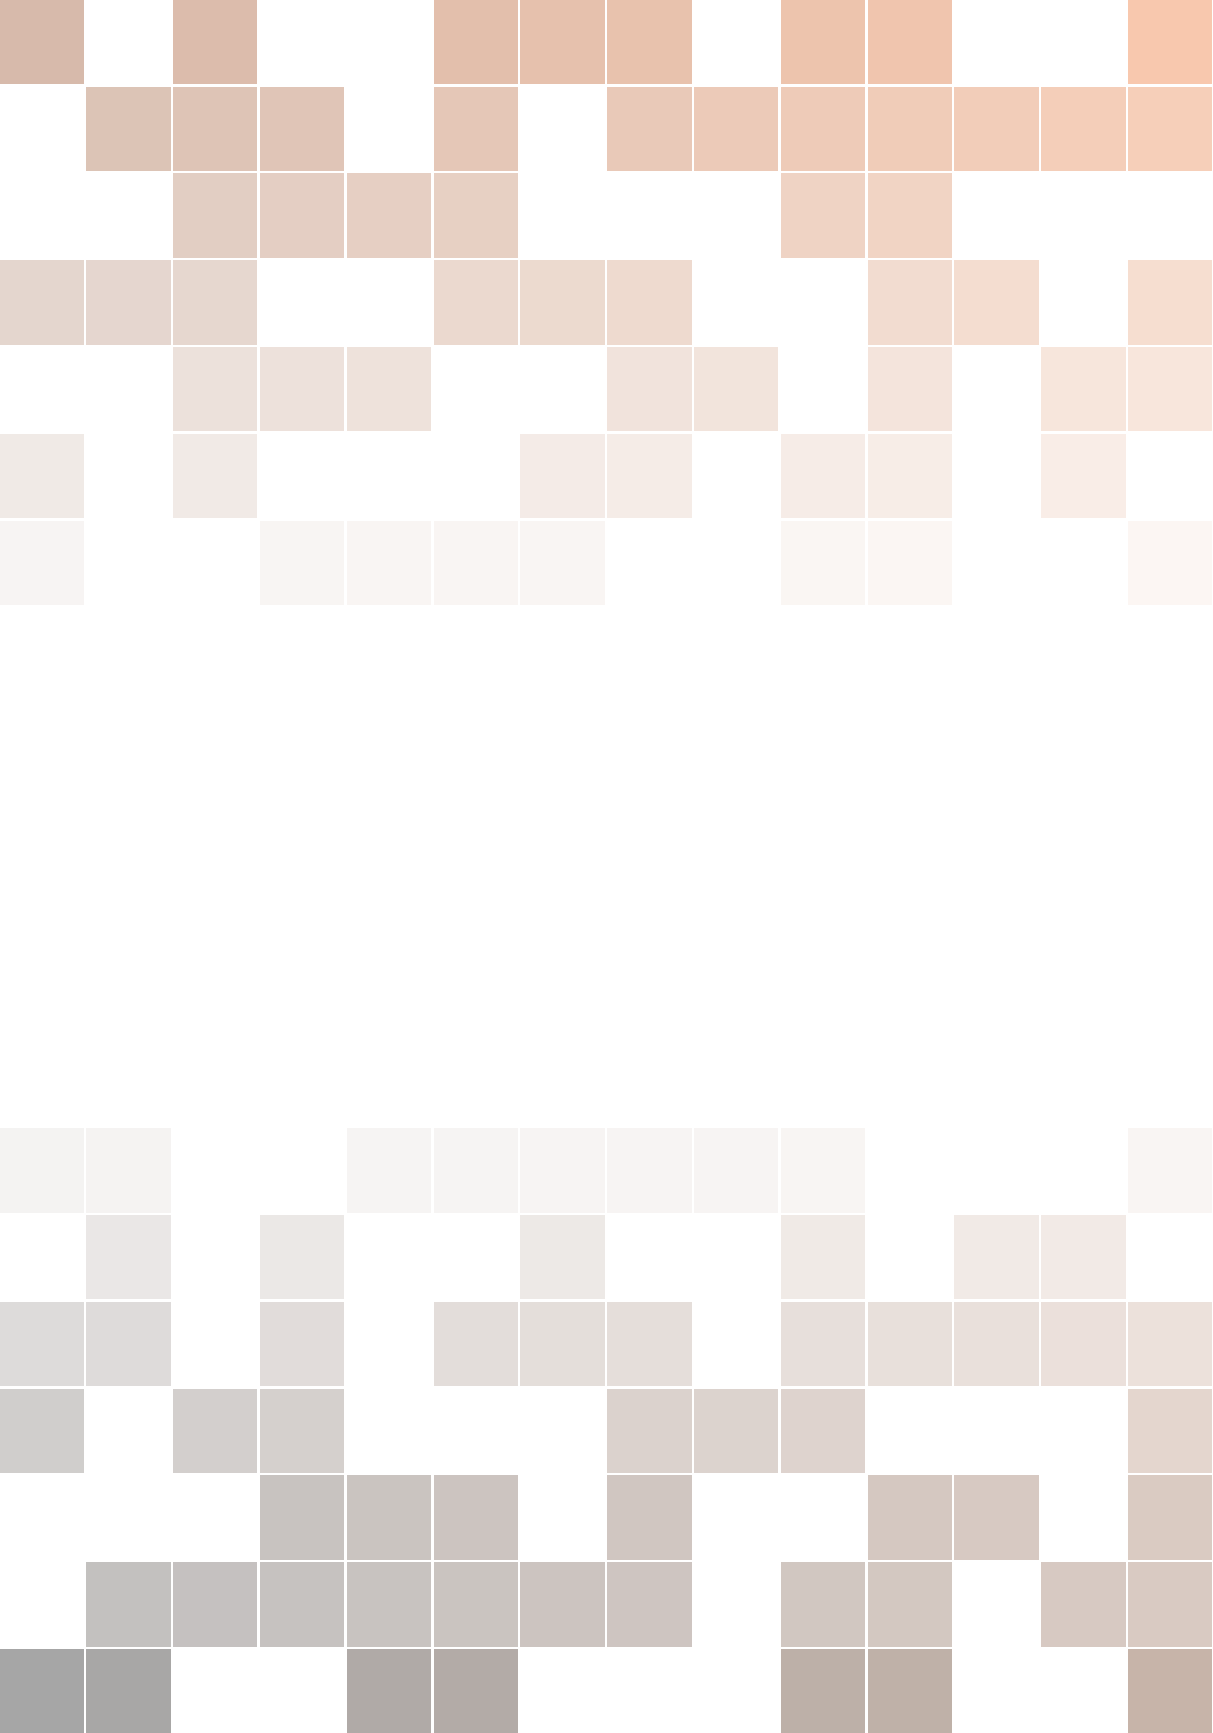
\includegraphics[scale=1]{background}}} % Image background
\centering
\vspace*{9cm}
\par\normalfont\fontsize{35}{35}\sffamily\selectfont
Práctica Final Ingeniería del Conocimiento\par % Book title
\vspace*{1cm}
{\large María Cristina Heredia Gómez}\par % Author name
{\large Alejandro Alcalde Barros}\par % Author name

{\footnotesize ETSs para hombres}\par

\endgroup

%----------------------------------------------------------------------------------------
%	COPYRIGHT PAGE
%----------------------------------------------------------------------------------------

\newpage
~\vfill
\thispagestyle{empty}

\noindent Copyright \copyright\ 2015 \\ % Copyright notice

\noindent \textit{\today} % Printing/edition date

%----------------------------------------------------------------------------------------
%	TABLE OF CONTENTS
%----------------------------------------------------------------------------------------

\chapterimage{chapter_head_1} % Table of contents heading image

\pagestyle{empty} % No headers

\tableofcontents % Print the table of contents itself

\cleardoublepage % Forces the first chapter to start on an odd page so it's on the right

\pagestyle{fancy} % Print headers again

%----------------------------------------------------------------------------------------
%	CHAPTER 1
%----------------------------------------------------------------------------------------

\chapterimage{chapter_head_1} % Chapter heading image

\chapter{Esquema de razonamiento}

\section{Esquema de razonamiento}\index{Esquema de razonamiento}

\section{Reglas indicadas en mi función como experto}\index{reglas}

This statement requires citation \cite{book_key}; this one is more specific \cite[122]{article_key}.

Lists are useful to present information in a concise and/or ordered way\footnote{Footnote example...}.

\subsection{Numbered List}\index{Lists!Numbered List}
\subsection{Bullet Points}\index{Lists!Bullet Points}
\subsection{Descriptions and Definitions}\index{Lists!Descriptions and Definitions}


%----------------------------------------------------------------------------------------
%	CHAPTER 2
%----------------------------------------------------------------------------------------

\chapterimage{chapter_head_1} % Chapter heading image

\chapter{Procedimiento seguido}

\section{Sesiones con el experto}\index{Prodecimiento!Sesiones}

Para el desarrollo de este sistema se han necesitado de 18 sesiones con el experto, de unos 30-40 minutos. Repartidas como sigue:

\begin{itemize}
  \item 7 sesiones para obtener el conocimiento.
  \item 6 para diseñar y representar la información, y la relación de síntomas con enfermedades.
  \item 4 sesiones se dedicaron a mostrar el prototipo del sistema experto al cliente, para corregir y retocar lo necesario.
  \item Las 2 sesiones restantes se dedicaron a validad y verificar.
\end{itemize}

\section{Procedimiento de validación y verificación}\index{Prodecimiento!validación}\index{Prodecimiento!verificación}

\subsection{Verificación}
\label{sub:Verificación}

Para la verificación de este sistema experto, ha sido necesario un proceso mediante el cual se han contemplado las tareas de \textbf{verificación del cumplimiento de especificaciones}, \textbf{verificiación de mecanismos de inferencia}, y \textbf{verificación de la base de conocimientos}.

Para verificar el cumplimento de las especificaciones, el sistema ha sido probado para todos los posibles casos tanto por la desarrolladora como por el experto, y un pequeño grupo de 5 usuarios independientes.\\ \\Para ésto, se han contemplado rasgos como que el conocimiento se haya representado adecuadamente,  que la forma de razonar del sistema haya sido la adecuada, que el sistema haya sido diseñado de forma modular, que la interfaz de usuario cumpla las especificaciones, que se cumplan los requitisitos de rendimiento.
\\
La verificación de los mecanismos de inferencia, ha sido realizada por la desarrolladora de la herramienta (el ingeniero del conicimiento), tratando de verificar el funcionamiento correcto del sistema sometiéndolo a distintas pruebas.
\\
Por último, la verificación de la base de conocimientos ha sido realizada únicamente por el ingeniero del conocimiento, buscando anomalías que no constituyan errores (y errores que no constituyan anomalías). Para ello, se han evaludado aspectos como la consistencia y la completitud. Se ha comprobado que en el sistema no hay reglas con incertidumbre, que no hay redundancia y que apenas se usen sentencias \textbf{IF}, así como que no haya reglas sin salida o reglas inalcanzables.\\ \\Con este proceso de verificación no buscamos que las respuestas del sistema sean correctas(validación), sino comprobar que el diseño y la implementación del sistema son correctos. \\
\subsection{Validación}
\label{sub:Validación}

Validar el sistema supone analizar si los resultados son correctos y si se cumplen las necesidades y los requisitos del usuario.

El personal involucrado en la validación ha sido el ingeniero de conocimiento, ya que es quién mejor conoce el sistema, el experto y un grupo de evaluadores independientes.

La estructura del razonamiento ha sido correctamente validada a lo largo de todo el desarrollo, comprobando que en cada momento el sistema alcanzaba una respuesta coherente con los datos introducidos por el usuario. Así, el sistema razonaba en base al problema presentado por el usuario, y lo aconsejaba.

% Datos usados en la validación
Ya que no se disponían de datos suficientes, se ha intentado mantener la representatividad basándonos en un documento suministrado, en el cual se indicaban las probabilidades de padecer una enfermedad.

% Criterios de validación
El criterio de validación seguido a sido un sistema de validación contra el experto. El sistema se ha construido con el conocimiento de un solo experto, luego, es ese mismo experto el que evalua el sistema. La desventaja de este método es algo subjetivo.


% Momento  en el que realizar la validación
Aunque ésta decisión suele ser algo controvertida, en éste caso se ha realizado la validación a lo largo de todo el proceso de desarrollo. Cada vez que se añadían nuevas reglas, o conocimiento, se ejecutaba para comprobar que las salidas del sistema eran las esperadas. Una vez finalizado, también se realizó una validación completa.

% Métodos de validación
El método de validación usado ha sido \textbf{análisis de sensibilidad}, en el cual se introducen al sistema casos muy similares entre sí, con diferencias muy pequeñas entre sí, y el sistema dará respuestas distintas.

% Errores en la validación
No se ha encontrado ningún error de tipo 2 en el sistema, ya que se ha comprobado que toda salida proporcionada es coherente con los datos introducidos por el usario.


%----------------------------------------------------------------------------------------
%	CHAPTER 3
%----------------------------------------------------------------------------------------

\chapterimage{chapter_head_1} % Chapter heading image

\chapter{Descripción del sistema desarrollado}


\section{Variables de entrada}\index{Sistema!Variables entrada}

Las variables de entrada serán todas las preguntas a las que vaya respondiendo el usuario, en éste caso se reponde mediante la selección de números.

Las respuestas de tipo si/no, se representan  mediante un 0 para el no, y un 1 para el sí. Cuando se le presenta al usuario un menu, las opciones de éste están enumeradas, y se seleccionará el elemento introduciendo su número correspondiente.

\section{Variables de salida}\index{Sistema!Variables salida}

Como variables de salida de nuestro sistema, tenemos la información que se muestra al usuario, en función de las entradas que ha realizado.

\section{Conocimiento global}\index{Sistema!Conocimiento global}

% El conociemiento global se ha representado mediante las siguientes relaciones de enfermedades con síntomas.

El conocimiento global se ha dividido en dos partes, el conocimiento cargado en el sistema inicialmente, y el asertado a medida que el usuario interactua con el sistema.

\begin{newlispcode}
  (deftemplate std "Template representing a STD"
      (slot std-name)
      (slot std-symtom)
      (slot std-symtom-where)
  )

  ;; Facts
  (deffacts Kwnoledge
    (std
      (std-name uretritis) (std-symtom inflamacion) )
    (std
      (std-name uretritis) (std-symtom coagulo) )
    (std
      (std-name uretritis) (std-symtom calculos) )
    (std
      (std-name uretritis) (std-symtom fluido) )
    (std
      (std-name uretritis) (std-symtom dolor-testiculos) )

    (std
      (std-name proctitis) (std-symtom inflamacion-recto) )
    (std
      (std-name proctitis) (std-symtom dolor-anorectal) )
    (std
      (std-name proctitis) (std-symtom sangrado) )
    (std
      (std-name proctitis) (std-symtom extrenimiento) )
    (std
      (std-name proctitis) (std-symtom pus) )

    (std
      (std-name balanitis) (std-symtom ardor) )
    (std
      (std-name balanitis) (std-symtom infeccion) )

    (std
      (std-name infec-faringeas) (std-symtom dolor-garganta) )
    (std
      (std-name infec-faringeas) (std-symtom inflamacion-ganglios-linf) )

    (std
      (std-name balanitis) (std-symtom candidas) )
    (std
      (std-name balanitis) (std-symtom prurito) )
    (std
      (std-name balanitis) (std-symtom ardor) )

    (std
      (std-name faringeas) (std-symtom dolor-garganta) )
    (std
      (std-name faringeas) (std-symtom inflamacion-ganglios-linf) )

    (std
      (std-name ulcera-genital) (std-symtom inflamacion-ganglios-ingles) )

     (std
      (std-name ulcera-genital) (std-symtom erupcion-pustula) )

    (std
      (std-name ectoparasitosis) (std-symtom macula-roja) )
    (std
      (std-name ectoparasitosis) (std-symtom liendres-ladillas) )

    ;; Sífilis prematura
    (std
      (std-name sifilis) (std-symtom ulcera) )

    ;;Sífilis secundaria
    (std
      (std-name sifilis) (std-symtom roseola-rosa-palida-tronco) )
    (std
      (std-name sifilis) (std-symtom rojo-oscuro-platas) )
    (std
      (std-name sifilis) (std-symtom rojo-oscuro-zona-humeda) )
    (std
      (std-name sifilis) (std-symtom alopecia) )
  )
\end{newlispcode}

\section{Módulos desarrollados}\index{Sistema!Módulos}

Se han definido cinco modulos:
\begin{itemize}
  \item El principal, donde se decide qué tipo de usuario está interactuando con el sistema. Su objetivo es dar a conocer al sistema ante qué tipo de usuario se enfrenta. No usa conocimiento.
  \item Módulo inflamaciones, en el que se tratan todas las enfermedades relacionadas con sintomas inflamatorios. En él, se van haciendo preguntas para descartar o asertar qué posible enfermedad puede padecer el usuario. El objetivo es decidir qué tipo de enfermedad inflamatoria puede padecer el usuario.
  \item Módulo para la faringitis, contempla los síntomas posibles para las faringitis. Su objetivo es deducir qué tipo de faringitis padece el usuario.
  \item Úlceras, Contempla los síntomas de las distintas úlceras, y decidirá qué tipo de ellas padece el usuario, de ser así. El objetivo es decidir qué tipo de úlcera padece el usuario.
  \item Un módulo de información, que se usará cuando se llegue a la conclusión de qué puede padecer el usuario, o se mostrará información para el usuario de tipo 3. En éste módulo, el objetivo es motrar la información necesaria en base a lo deducido en los módulos anteriores.
\end{itemize}

\section{Estructura del esquema de razonamiento}\index{Sistema!Esquema razonamiento}

El modulo principal es el que se ejecuta al iniciar el sistema experto. Si el usuario usando el sistema es de tipo 1, el modulo de inflamaciónes intentará buscar una enfermedad que corresponda con sus síntomas, de no encontrarla, se pasará al módulo de faringitis, luego al de úlceras y finalmente al de información.\\
Al usuario de tipo 2 se le harán una serie de preguntas para determinar el por qué de su preocupación, una vez obtenido ese conocimiento, se pasará por el módulo correspondiente en función de sus respuestas.\\
Al usuario de tipo 3 se le pregunta por qué tipo de enfermedad quiere informarse, y se ejecuta directamente el módulo de información basándose en su respuesta.

\section{Lista de hechos usada durante ejecución}\index{Sistema!Lista de hechos}

Hay dos tipos de hechos que se asertan durante la ejecución del sistema, unos representan qué opción ha elegido el usuario al interactuar, por ejemplo, si se presenta un menú de 3 elementos, se asertará un hecho, por ejemplo \newlispinline/(nombre-hecho-para-menu ?respuesta-menu)/, donde \newlispinline/?respuest-menu/ será un número que represente la opción elegida.\\
El otro tipo de hecho representa conocimiento deducido por el sistema, por ejemplo \newlispinline/(assert (infoUlceraMala) )/ significa que el sistema ha deducido que el usuario debería informarse sobre el tipo de úlcera asertado.

\section{Reglas de cada módulo}\index{Sistema!Reglas}

Para el módulo de faringitis:
\begin{itemize}
  \item Si ha practicado sexo oral, con una o varias personas y alguna de ellas ha dado positivo en alguna ETS, es probable que los síntomas de su faringitis vengan dados por una ETS. De lo contrario, lo más probable es que padezca una faringitis de repetición (Una faringitis normal).
\end{itemize}

Para el caso de las úlceras\index{reglas!úlceras} hay que contemplar varios aspectos.
\begin{itemize}
  \item Lás úlceras graves son más probables de transmitirse en paises tropicales. Por tanto, si el usuario no ha estado en contacto con una persona de esos paieses, o no los ha frecuentado, es poco probable que se haya contagiado.
  \item Para contemplar la sífilis, en caso de que se haya estado en contacto con alguien de paises tropicales, o en paieses tropicales, las reglas son las siguientes:
  \begin{itemize}
    \item Si tiene una úlcera color rosa pálido, es probable que tenga Roseola Sifílica, un tipo de sífiles secundaria, de las más comunes y precoces.
    \item Si tiene una úlcera color rojo oscuro, en el tronco o extremidades, planta o palma, lo más probable es que padezca Sifilides Papulosa, otro tipo de sífilis secundaria.
    \item Si tiene una úlcera roja oscura, pero en el area genital, perineo, ingles, axilas, o zonas húmedas o de plieges, es probable que padezca Condilomas Planos, otro tipo de sífiles secundaria. Aparece a los 3-6 meses de la infección.
    \item Si padece caida del pelo por zonas, o en placas, puede padecer Alopecia Sifílica.
  \end{itemize}
  \item En las verrugas genitales, Si ha tenido una relación de riesgo, es probable que tenga una.
  \item En el caso de las ectoparasitosis:
  \begin{itemize}
    \item Si le pica la zona, y ha tenido una relación de riesgo, es posible que tenga liendres.
    \item Si ha tenido una relación de riesgo, pero no le pica, lo más probable es que tenga prurito.
  \end{itemize}
  \item Las reglas para las enfermedades relacionadas con las inflamaciones son:
  \begin{itemize}
    \item Si presenta síntomas con fluidos amarillentos, posiblemente tenga uretritis.
    \item Si presenta tenesmo y/o sangrado rectal, es probable que tenga proctitis.
    \item Cuando el usuario tiene escozor y ardor tras el coito, hay una alta probabilidad de que tenga balanitis.
  \end{itemize}
\end{itemize}


%----------------------------------------------------------------------------------------
%	CHAPTER 4
%----------------------------------------------------------------------------------------

\chapterimage{chapter_head_1} % Chapter heading image

\chapter{Manual de uso}


%----------------------------------------------------------------------------------------
%	INDEX
%----------------------------------------------------------------------------------------

\cleardoublepage
\setlength{\columnsep}{0.75cm}
\addcontentsline{toc}{chapter}{\textcolor{ocre}{Index}}
\printindex

%----------------------------------------------------------------------------------------

\end{document}
